\documentclass{beamer}
\usetheme{STCE}

\usepackage{beamerfoils}
\usepackage[utf8]{inputenc}
\usepackage{amsmath}
\usepackage[german]{babel} % Für deutche Umlaute
\usepackage{tabularx} % Für die TabularX Umgebung

\MyLogo{
\centering

\includegraphics[width=0.12\textwidth]{figures/logo.eps}
}

\begin{document}
\title{Correlation and Regression Analysis\\
TEACH}
\author{Patrick Neidig \and Marius Grysla}
\institute{Software and Tools for Computational Engeneering}
\date{31.5.2011}
\frame{\titlepage}

\begin{frame}
 \frametitle{Inhalt}
 \tableofcontents
\end{frame}

\section{Beispiel}

\begin{frame}
	\frametitle{Beispiel: Münchner Mietspiegel 2003}
	
	\begin{block}{Begriff: Mietspiegel}
		stellt Mietern, Vermietern und Mietberatungsstellen eine Orientierungshilfe bei Mietfragen und insbesondere der Ermittlung der 	ortsüblichen  Vergleichsmiete (Nettomiete in Abhängigkeit der Größe, Art, Ausstattung, Beschaffenheit und Lage der Wohnung) zur Verfügung
	\end{block}
	
	\begin{itemize}
		\item Ausschnitt (2053 Fälle) aus Münchens Mietspiegel im Jahr 2003
		\item repräsentative Zufallsstichprobe aus der Gesamtheit aller Wohnungen
		\item interessierende Daten von Interviewern mit Hilfe von Fragebögen ermittelt
	\end{itemize}
\end{frame}

\begin{frame}
	\frametitle{Beispiel: Münchner Mietspiegel 2003}
	
	\par \textbf{Übersicht der Variablen}\\[3mm]
	
	\begin{tabular}[ht]{|l|l|l|}
  	\hline
  	\textit{Name} & \textit{Beschreibung} & \textit{Skalenniveau}\\
  	\hline \hline
  	nm & Nettomiete in Euro & verhältnisskaliert\\ \hline
  	nmqm & Nettomiete pro Quadratmeter in Euro & verhältnisskaliert\\ \hline
  	wfl & Wohnfläche in Quadratmeter & verhältnisskaliert\\ \hline
  	rooms & Anzahl der Zimmer & verhältnisskaliert\\ \hline
  	bj & Baujahr & intervallskaliert\\ \hline
  	bez & Stadtbezirk & nominalskaliert\\ \hline
  	wohngut & gute Wohnlage & dichotom\\ \hline
  	wohnbest & beste Wohnlage & dichotom\\ \hline
  	... & diverse Variablen zur Ausstattung & dichotom\\
  	\hline
	\end{tabular}
\end{frame}

\begin{frame}
	\frametitle{Beispiel: Münchner Mietspiegel 2003}
	
	\par \textbf{Reduzierter Datensatz (8 Fälle ohne Variablen zur Ausstattung)}\\[3mm]
	
	\begin{tabular}[ht]{|l|l|l|l|l|l|l|l|}
  	\hline
  	\textit{nm} & \textit{nmqm} & \textit{wfl} & \textit{rooms} & \textit{bj} & \textit{bez} & \textit{wohngut} & \textit{wohnbest}\\
  	\hline \hline
  	214,14 & 5,95 & 36 & 2 & 1948 & 17 & 0 & 0\\ \hline
  	406,93 & 6,26 & 65 & 2 & 1966 & 10 & 0 & 0\\ \hline
		603,34 & 7,64 & 79 & 3 & 1986 & 13 & 1 & 0\\ \hline
		826,26 & 8,88 & 93 & 3 & 1918 & 5 & 1 &0\\ \hline
		1000,41 & 9,81 & 102 & 3 & 1918 & 8 & 0 & 0\\ \hline
		1227,12 & 10,14 & 121 & 5 & 1924 & 9 & 1 & 0\\ \hline
		1385,12 & 10,82 & 128 & 6 & 1991 & 9 & 1 & 0\\ \hline
		1661,55 & 11,08 & 150 & 5 & 1966 & 13 & 0 & 0\\
  	\hline
	\end{tabular}
\end{frame}

\section{Korrelation}

\subsection{Funktion der NAG Library}

\begin{frame}
	\frametitle{Korrelation: Funktion der NAG Library}
	
	\par \textbf{Spezifikation}\\[3mm]
	
	\par void nag\_corr\_cov (Integer $n$, Integer $m$, const double $x[]$, Integer $tdx$,
	\hspace*{5mm} const Integer $sx[]$, const double $wt[]$, double *$sw$, double $wmean[]$,
	\hspace*{5mm} double $std[]$, double $r[]$, Integer $tdr$, double $v[]$, Integer $tdv$,
	\hspace*{5mm} NagError *$fail$)
	
	\begin{itemize}
		\item Korrelationskoeffizient nach Bravais und Pearson
	\end{itemize}
\end{frame}

\begin{frame}
	\frametitle{Korrelation: Funktion der NAG Library}
	
	\par \textbf{Übersicht der Input-Argumente}\\[3mm]
	
	\begin{tabular}[ht]{|l|p{9cm}l|}
  	\hline
  	\textit{Name} & \textit{Beschreibung}\\
  	\hline \hline
  	$n$ & Anzahl der Fälle im Datensatz ($n > 1$)\\ \hline
  	$m$ & Anzahl der Variablen im Datensatz ($m \geq 1$)\\ \hline
        $x[n \times tdx]$ & Datenmatrix: $x[i - 1][j - 1]$ enthält \newline
        den $i$-ten Fall der $j$-ten Variable\\ \hline
        $tdx$ & Zeilenlänge der Datenmatrix $x$ ($tdx \geq m$)\\ \hline
        $sx[m]$ & gibt für jede Variable an, ob sie in die Analyse einbezogen wird: einbezogen falls $sx[j] > 0$, sonst nicht ($sx[j] \geq 0$)\\ \hline
        $wt[m]$ & gibt für jeden Fall eine Gewicht an ($wt[i] \geq 0$)\\ \hline
        $sw$ & Summe der Gewichte falls $wt$ gesetzt, sonst gleich $n$\\ \hline
        $tdr$, $tdv$ & beide analog zu $tdx$\\
  	\hline
	\end{tabular}
\end{frame}

\begin{frame}
	\frametitle{Korrelation: Funktion der NAG Library}
	
	\par \textbf{Übersicht der Output-Argumente}\\[3mm]
	
	\begin{tabular}[ht]{|l|p{9cm}l|}
  	\hline
  	\textit{Name} & \textit{Beschreibung}\\
  	\hline \hline
  	$wmean[m]$ & Erwartungswerte: $wmean[j - 1]$ enthält \newline
  	den Erwartungswert für die $j$-te Variable\\ \hline
  	$std[m]$ & Standardabweichungen: $std[j - 1]$ enthält \newline
  	die Standardabweichung für die $j$-te Variable\\ \hline
		$r[n \times tdr]$ & Korrelationsmatrix: $r[j - 1][k - 1]$ enthält \newline
		den Korrelationskoeffizienten nach Bravais \newline
		und Pearson für die Variablen $j$ und $k$\\ \hline
		$v[n \times tdv]$ & Kovarianzmatrix: $v[j - 1][k - 1]$ enthält \newline
		die Kovarianz zwischen den Variablen $j$ und $k$\\
  	\hline
	\end{tabular}
\end{frame}

\subsection{Algorithmus der Funktion}

\begin{frame}
	\frametitle{Korrelation: Algorithmus der Funktion}

	\begin{block}{Frage}
		Welche Variablen haben Einfluss auf die Nettomiete?
	\end{block}
	
	\begin{itemize}
		\item intuitive Lösung durch Streudiagramme
		\begin{itemize}
			\item falls die Wertepaare der ausgewählten Variable und der Nettomiete zu einer Geraden positiver/negativer Steigung tendieren, liegt ein linearer Zusammenhang und somit eine positive/negative Korrelation vor
			\item ist keine solche Tendenz zu sehen, liegt keine Korrelation vor
		\end{itemize}
	\end{itemize}
\end{frame}

\begin{frame}
	\frametitle{Korrelation: Algorithmus der Funktion}
	
	\begin{center}
    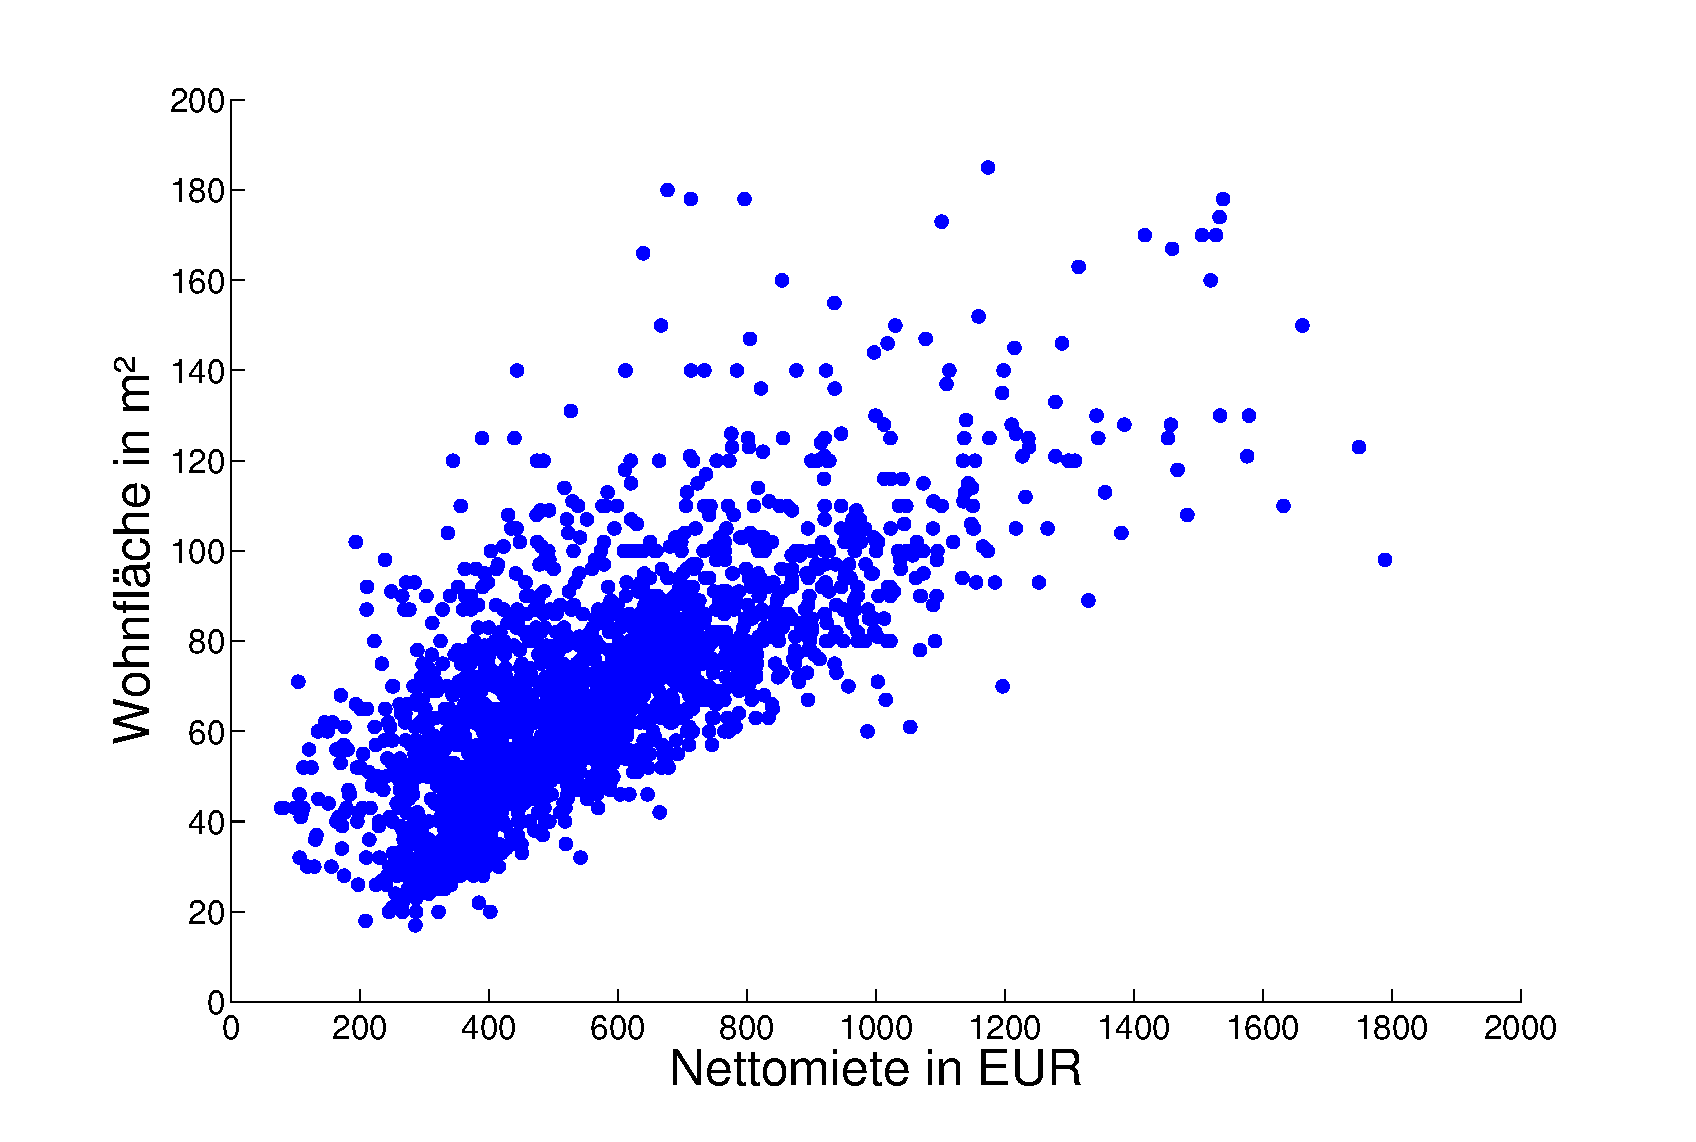
\includegraphics[width=11cm]{figures/streudiag-nm-wfl-alle}
  \end{center}
\end{frame}

\begin{frame}
	\frametitle{Korrelation: Algorithmus der Funktion}
	
	\begin{center}
    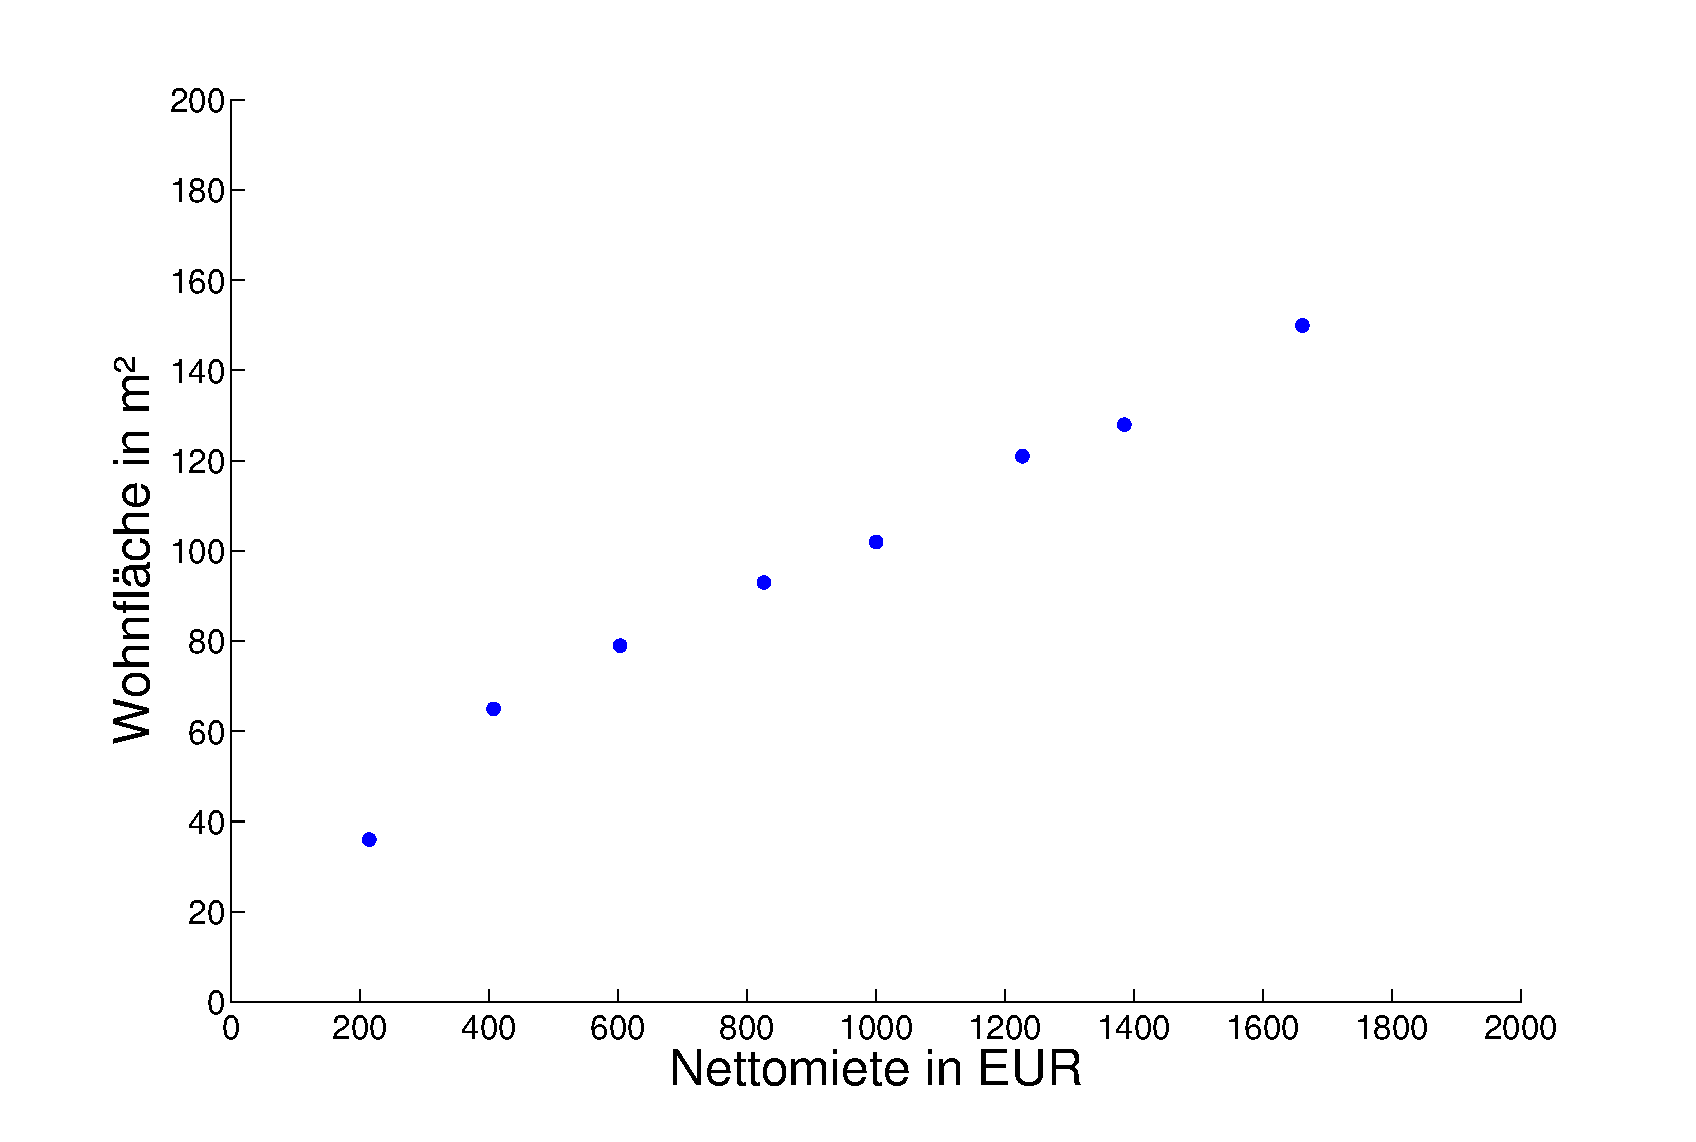
\includegraphics[width=11cm]{figures/streudiag-nm-wfl-red}
  \end{center}
\end{frame}

\begin{frame}
	\frametitle{Korrelation: Algorithmus der Funktion}
	
	\begin{center}
    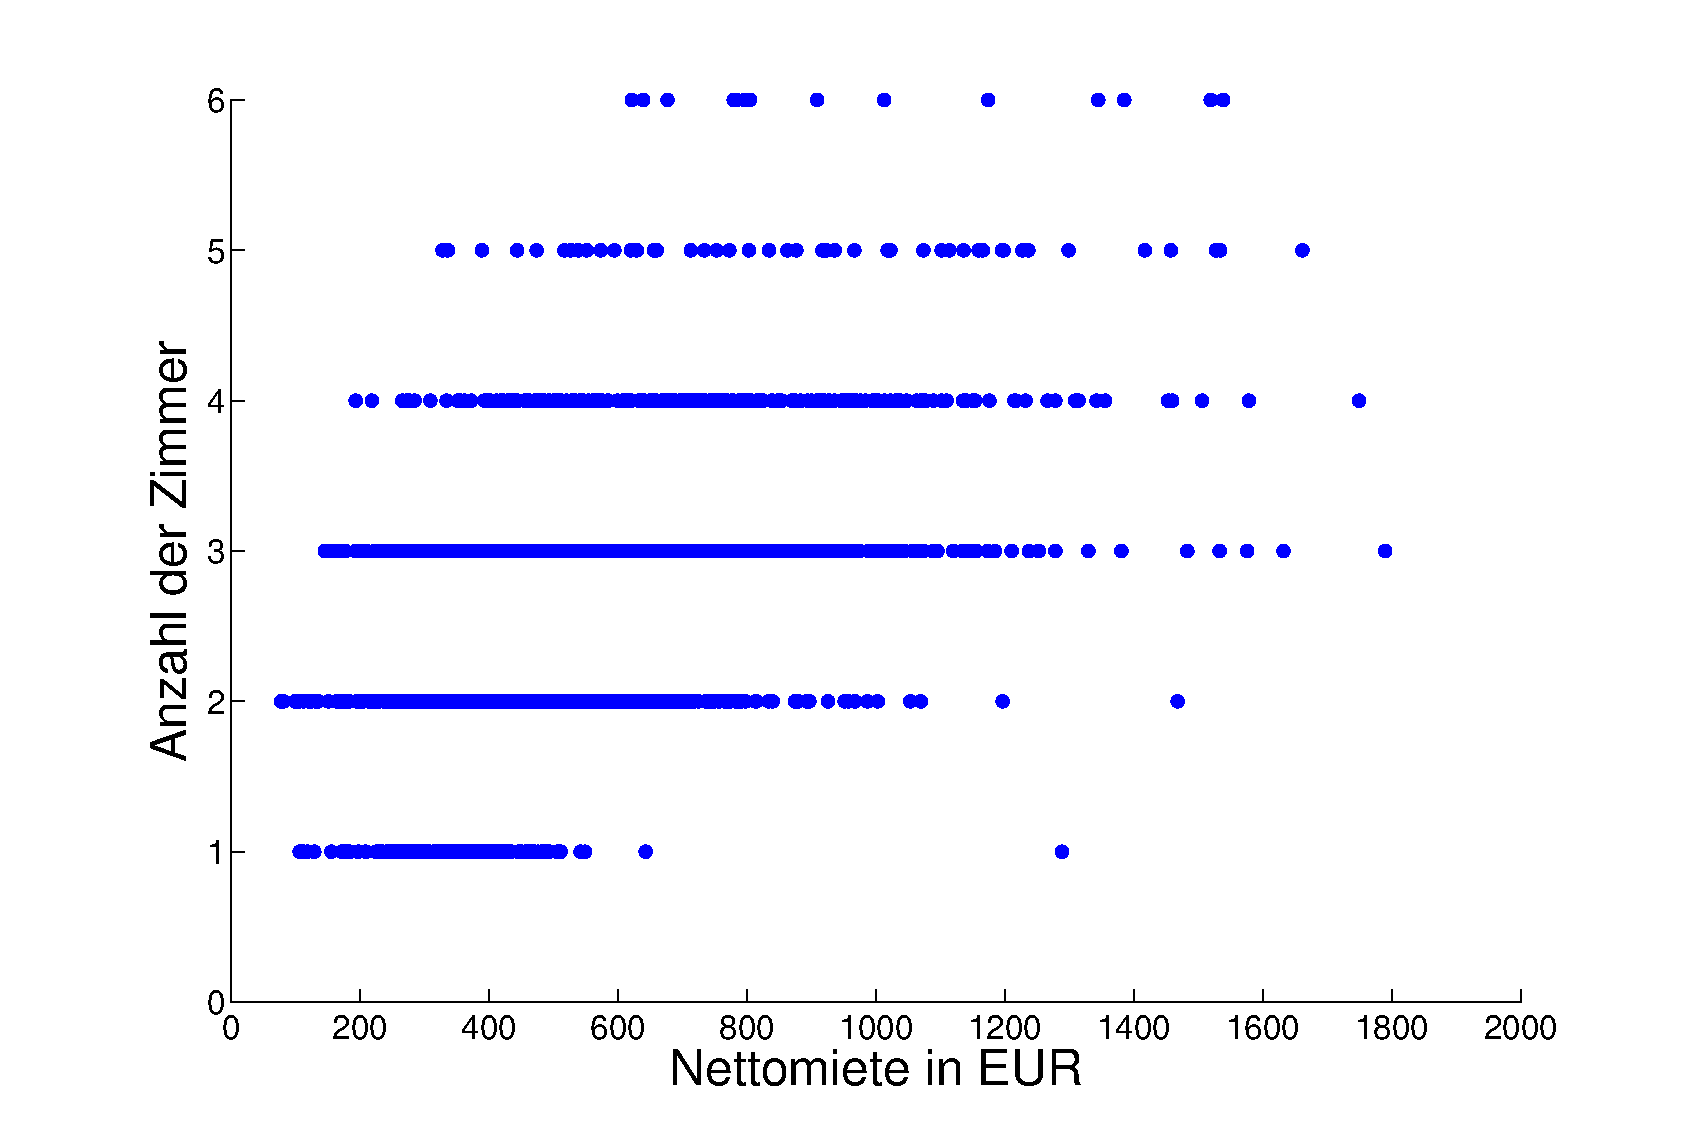
\includegraphics[width=11cm]{figures/streudiag-nm-rooms-alle}
  \end{center}
\end{frame}

\begin{frame}
	\frametitle{Korrelation: Algorithmus der Funktion}

	\begin{block}{Problem}
		Streudiagramme sind offensichtlich sehr ungenau und können nicht in jedem Fall Auskunft über die Korrelation geben.
	\end{block}

	\begin{itemize}
		\item genauere Lösung durch Algorithmus
		\begin{itemize}
			\item Eingabe: komplette Datenmatrix mit allen Variablen und Fällen
			\item sukzessive Berechnung der Erwartungswerte und Standardabweichungen für alle Variablen sowie Berechnung der Kovarianzmatrix
			\item abschließende Berechnung der Korrelationsmatrix (enthält die Korrelationskoeffizienten für alle Variablenpaare)
			\item Ausgabe: alle oben berechneten Werte
		\end{itemize}
	\end{itemize}
\end{frame}

\begin{frame}
	\frametitle{Korrelation: Algorithmus der Funktion}

	\par \textbf{1. Schritt: Erwartungswerte berechnen}\\[3mm]
	
	\begin{itemize}
		\item hier: analog zur Berechnung des arithmetischen Mittelwerts, da keine Gewichtung der Fälle vorgenommen wird
	\end{itemize}
	
	\begin{block}{Formel: Arithmetischer Mittelwert}
		\begin{equation*}
			\bar{x}=\dfrac{1}{n}\sum_{i=1}^{n}{x_i}=\dfrac{1}{n}(x_1+...+x_n)
		\end{equation*}
	\end{block}
\end{frame}

\begin{frame}
	\frametitle{Korrelation: Algorithmus der Funktion}

	\begin{block}{Reduziertes Beispiel}
	  $X$ := Nettomiete
		\begin{equation*}
			\bar{x}=\dfrac{1}{8}(214,14+406,93+603,34+826,26+...+1661,55)=915,61
		\end{equation*}
	\end{block}
	
	\begin{itemize}
		\item wird für alle Variablen der eingegebenen Datenmatrix (Nettomiete, Wohnfläche, Zimmer etc.) separat berechnet
	\end{itemize}
\end{frame}

\begin{frame}
	\frametitle{Korrelation: Algorithmus der Funktion}

	\par \textbf{2. Schritt: Standardabweichungen berechnen}\\[3mm]
	
	\begin{block}{Formel: Standardabweichung}
		\begin{equation*}
			s_X=\sqrt{\dfrac{1}{n}\sum_{i=1}^{n}{(x_i-\bar{x})^2}}=\sqrt{\dfrac{1}{n}(x_1-\bar{x})^2+...+(x_n-\bar{x})^2}
		\end{equation*}
	\end{block}
\end{frame}

\begin{frame}
	\frametitle{Korrelation: Algorithmus der Funktion}

	\begin{block}{Reduziertes Beispiel}
	  $X$ := Nettomiete
		\begin{equation*}
			s_X=\sqrt{\dfrac{1}{8}(214,14-915,61)^2+...+(1661,55-915,61)^2}=466,02
		\end{equation*}
	\end{block}
	
	\begin{itemize}
		\item wird ebenfalls für alle Variablen separat berechnet
	\end{itemize}
\end{frame}

\begin{frame}
	\frametitle{Korrelation: Algorithmus der Funktion}

	\par \textbf{3. Schritt: Kovarianzmatrix berechnen}\\[3mm]
	
	\begin{block}{Formel: Kovarianz}
		\begin{equation*}
			s_{XY}=\dfrac{1}{n}\sum_{i=1}^{n}{(x_i-\bar{x})(y_i-\bar{y})}=\dfrac{1}{n}(x_1-\bar{x})(y_1-\bar{y})+...+(x_n-\bar{x})(y_n-\bar{y})
		\end{equation*}
	\end{block}
\end{frame}

\begin{frame}
	\frametitle{Korrelation: Algorithmus der Funktion}

	\begin{block}{Reduziertes Beispiel}
	  $X$ := Nettomiete, $Y$ := Wohnfläche
		\begin{equation*}
				\begin{align*}
				s_{XY}=&\dfrac{1}{8}(214,14-915,61)(36-96,75)+...\\
				&+(1661,55-915,61)(150-96,75)=18147,94
				\end{align*}
		\end{equation*}
	\end{block}
	
	\begin{itemize}
		\item wird für alle Variablen paarweise berechnet
	\end{itemize}
\end{frame}

\begin{frame}
	\frametitle{Korrelation: Algorithmus der Funktion}

	\par \textbf{4. Schritt: Korrelationsmatrix berechnen}\\[3mm]
	
	\begin{block}{Formel: Korrelationskoeffizient nach Bravais und Pearson}
		\begin{equation*}
			r=\dfrac{s_{XY}}{s_Xs_Y}=\dfrac{\sum_{i=1}^{n}{(x_i-\bar{x})(y_i-\bar{y})}}{\sqrt{\sum_{i=1}^{n}{(x_i-\bar{x})^2\sum_{i=1}^{n}{(y_i-\bar{y})^2}}}}
		\end{equation*}
	\end{block}
	
	\begin{itemize}
		\item wird ebenfalls für alle Variablen paarweise berechnet
	\end{itemize}
\end{frame}

\begin{frame}
	\frametitle{Korrelation: Algorithmus der Funktion}
	
	\par \textbf{Beispiel}

	\begin{equation*}
		R =
		\begin{footnotesize}
			\begin{pmatrix}
				1.00 & 0.47 & \textcolor{red}{0.71} & \textcolor{red}{0.54} & 0.05 & -0.07 & 0.16 & 0.15\\
   			0.47 & 1.00 & -0.23 & -0.27 & 0.29 & -0.07 & 0.15 & 0.11\\
  	 		0.71 & -0.23 & 1.00 & \textcolor{red}{0.84} & -0.20 & -0.05 & 0.09 & 0.06\\
	   		0.54 & -0.27 & 0.84 & 1.00 & -0.15 & 0.03 & 0.00 & 0.03\\
  	 		0.05 &  0.29 & -0.20 & -0.15 & 1.00 & 0.31 & -0.11 & 0.06\\
  			-0.07 & -0.07 & -0.05 & 0.03 & 0.31 & 1.00 & -0.31 & 0.06\\
				0.16 &  0.15 & 0.09 & 0.00 & -0.11 & -0.31 & 1.00 & -0.12\\
  			0.15 &  0.11 & 0.06 & 0.03 & 0.06 & 0.06 & -0.12 & 1.00\\
			\end{pmatrix}
		\end{footnotesize}
	\end{equation*}
\end{frame}

\subsection{Interpretation}

\begin{frame}
	\frametitle{Korrelation: Interpretation}

	Wertebereich $r$: $-1 \leq r \leq +1$
	\begin{itemize}
    \item $r>0$: positive Korrelation
    \item $r<0$: negative Korrelation
    \item $r=0$: keine Korrelation
	\end{itemize}
	Stärke der Korrelation:
	\begin{itemize}
    \item $|r|<0,5$: schwache Korrelation
    \item $0,5 \leq |r| < 0,8$: mittlere Korrelation
    \item $0,8 \leq |r|$: starke Korrelation
	\end{itemize}
\end{frame}

\section{Multiple Regression}

\subsection{Das Regressionsmodell}

\begin{frame}
 \frametitle{Das multiple lineare Regressionsmodell}
 \begin{itemize}
 \item Korrelationen:
   \begin{itemize}
   \item Verschiedene Merkmale haben einen Einfluß auf die Nettomiete
   \end{itemize}
 \item Offene Fragen:
   \begin{itemize}
   \item Mit welchem Aufpreis muss bei einer Wohnung in bester Wohnlage gerechnet werden?
   \item Hat das Baujahr einen Einfluss auf den Mietpreis/qm Verteilung?
   \end{itemize}
 \end{itemize}

 
\end{frame}



\begin{frame}
 \frametitle{Das multiple lineare Regressionsmodell}

 \begin{itemize}
  \item Wie groß sind die Einflüsse von verschiedenen Regressoren auf ein abhängiges Merkmal?
 \end{itemize}
 
 \begin{block}{Lineare Einfachregression}
  \begin{equation*}
   Y_i = \alpha + \beta x_i + \epsilon_i, \quad i = 1, \dots, n
  \end{equation*}
 \end{block}

 \begin{block}{Multiple Lineare Regression}
  \begin{equation*}
   Y_i = \beta_0 + \beta_1 x_{i1} + \dots + \beta_p x_{ip} + \epsilon_i, \quad i = 1, \dots, n
  \end{equation*}
  \begin{itemize}
   \item Anzahl der Regressoren: $p$
  \end{itemize}

 \end{block}

\end{frame}

\begin{frame}
  \frametitle{Verteilung Nettomieten}
  \begin{center}
    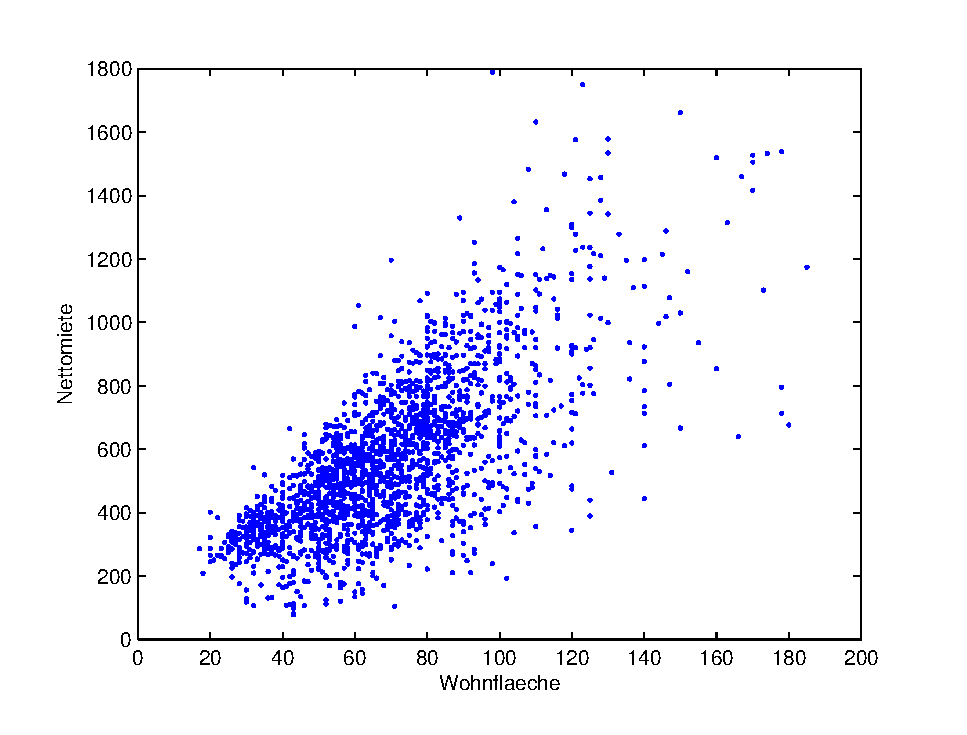
\includegraphics[width=10cm]{figures/nm_wfl_distribution}
  \end{center}
\end{frame}

\begin{frame}
  \frametitle{Verteilung Nettomieten II}
  \begin{center}
    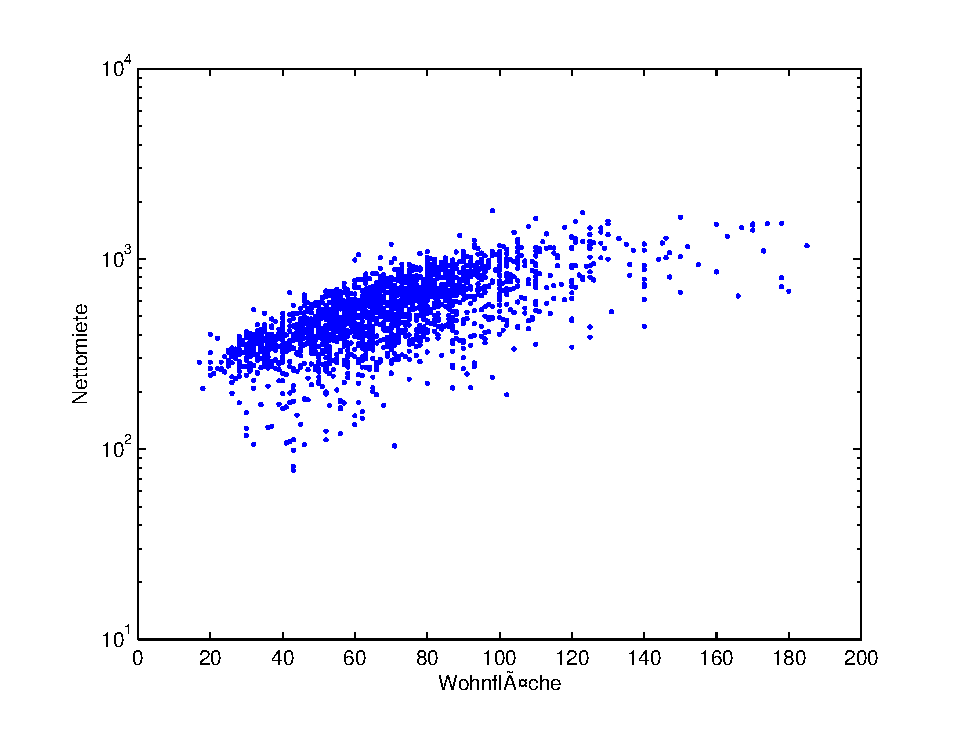
\includegraphics[width=10cm]{figures/nm_wfl_distribution_log}
  \end{center}
\end{frame}

\begin{frame}
  \frametitle{Anwendung}
  % Hier sollte die Verwendung der Regression mit dem Mietspiegel Beispiel verdeutlicht 
  
  % TODO: Welche Merkmale für Regression verwenden?
  %  - wohnfläche
  %  - wohnlage (gut, beste)
  %  - baujahr
  % TODO: Welche Zeilen auswählen

  \begin{itemize}
  \item Regressoren: Wohnfläche, gute Wohnlage, Baujahr
  \item Regressand: Nettomiete
  \end{itemize}

  \begin{block}{Regressionsansatz}
    \begin{equation*}
      log(NM) = \beta_0 + \beta_1 Wfl + \beta_2 Bj + \beta_3 gL + \epsilon
    \end{equation*}
  \end{block}

  % \begin{itemize}
  % \item Beispieldatensatz:\\
  %   \begin{tabular}[h]{c|c|c|c}
  %     1 & 2 & 3 & 4 \\
  %     5 & 6 & 7 & 8
  %   \end{tabular}
  % \end{itemize}

\end{frame}

\subsection{NAG Library Funktion}

\begin{frame}
  \frametitle{Multiple Regression: Funktionssignatur}
  
  \par \textbf{Spezifikation}\\[3mm]
  
  \par void nag\_regsn\_mult\_linear (Nag\_IncludeMean mean, Integer \alert<2>{$n$}, \linebreak
  \hspace*{5mm} const double \alert<2>{$x[]$}, Integer $tdx$, Integer \alert<2>{$m$}, const Integer \alert<2>{$sx[]$}, 
  \hspace*{5mm} Integer \alert<2>{$ip$}, const double \alert<2>{$y[]$}, const double $wt[]$, double \alert<3>{*$rss$}, \linebreak
  \hspace*{5mm} double *$df$, double \alert<3>{$b[]$}, double \alert<3>{$se[]$}, double $cov[]$, double \alert<3>{$res[]$},
  \hspace*{5mm} double $h[]$, double \alert<3>{$q[]$}, Integer $tdq$, Nag\_Boolean *$svd$, \linebreak
  \hspace*{5mm} Integer *$rank$, double $p[]$, double $tol$, double $com\_ar$, \linebreak
  \hspace*{5mm} NagError *$fail$)
    
  \begin{itemize}
  \item Führt eine generelle multiple lineare Regression aus.
  \end{itemize}

  %\par void nag\_regsn\_mult\_linear (Integer $n$, Integer $m$, const double $x[]$, Integer $tdx$,
  %\qquad const Integer $sx[]$, const double $wt[]$, double *$sw$, double $wmean[]$,
  %\hspace*{5mm} double $std[]$, double $r[]$, Integer $tdr$, double $v[]$, Integer $tdv$,
  %\hspace*{5mm} NagError *$fail$)
  
  %\begin{itemize}
  %\item Führt eine generelle multiple lineare Regression aus.
  %\end{itemize}

\end{frame}

\subsection{Berechnung der Funktion}

\begin{frame}
  \frametitle{NAG Algorithmus}
 
  \begin{block}{Für Berechnung wird eine Matrixschreibweise benötigt}
    {\centering $y = X \beta + \epsilon$ \\}
    wobei \\
    \qquad $y$ = Vektor mit $n$ Beobachtungen von $y$ \\
    \qquad $X$ = Matrix mit den Beobachtungen der Regressanden \\
    \qquad $\beta$ = Vektor mit unbekannten Faktoren \\
    \qquad $\epsilon$ = Vektor mit Fehlertermen \\
  \end{block}
  
  \pause
  
  \begin{block}{Methode der kleinsten Quadrate}
    In Matrixschreibweise:\\
    {\centering
      $\sum\limits^{N}_{n=1} \epsilon^2_n = \epsilon^T \epsilon = (y - X \beta)^T (y - X \beta) \rightarrow \min\limits_{\beta}$\\}
    oder: \\
    {\centering
      $\Vert X\beta - y \Vert_2 \rightarrow \min\limits_{\beta}$
      \\}
  \end{block}

\end{frame}



\begin{frame}
  \frametitle{QR-Zerlegung}
  
  \begin{itemize}
  \item Wie kann das benötigte Minimum berechnet werden?\\
    $\Rightarrow$ QR-Zerlegung der Matrix $X$
  \end{itemize}

  \begin{block}{QR-Zerlegung}
    Zerlegung von $X$ in zwei Matrizen $Q$ und $R$, sodass \\
    \qquad $Q$ ist orthogonale Matrix \\
    \qquad $R$ enthält obere Dreiecksmatrix \\
  \end{block}

  \pause

  \begin{itemize}
  \item Algorithmen:
    % Hier Vor-/Nachteile erwähnen
    \begin{itemize}
    \item Householder Transformationen 
    \item Givens Rotationen 
    \item Modifizierter Gram-Schmidt Algorithmus 
    \end{itemize}
  \end{itemize}

\end{frame}

\begin{frame}
  \frametitle{Householder Verfahren}
  \begin{block}{Householder Matrix}
    \[ P = I - 2vv^T / v^Tv \]    
    \begin{itemize}
    \item Erzeugt in einer Spalte $x$ Nullen
    \end{itemize}
  \end{block}
  
  \begin{itemize}
  \item Berechnung von $v$:\\
    $v = x / \beta,$\hspace{1cm} $v(1) = 1$ \\
    $\beta = x(1) + sign(x(1)) \|x\|_2$
  \end{itemize}

\end{frame}

\begin{frame}
  \frametitle{QR-Zerlegung (Beispiel)}
  $X = \small \begin{pmatrix}
    1	& 36	& 1948	& 0 \\
    1	& 65	& 1966	& 0 \\
    1	& 79	& 1986	& 1 \\
    1	& 93	& 1918	& 1 \\
    1	& 102	& 1918	& 0 \\
    1	& 121	& 1924	& 1 \\
    1	& 128	& 1991	& 1 \\
    1	& 150	& 1966	& 0 
  \end{pmatrix},$
  $x = \small \begin{pmatrix}
    1 \\ 1 \\ 1 \\ 1 \\ 1 \\ 1 \\ 1 \\ 1
  \end{pmatrix},$ 
  \pause
  $\beta = 3.83,$
  $v = \begin{pmatrix}
    1.00 \\ 0.26 \\ 0.26 \\ 0.26 \\ 0.26 \\ 0.26 \\ 0.26 \\ 0.26
  \end{pmatrix}$ \\

  \pause
  
  $(I - 2vv^T/v^Tv) X = \small \begin{pmatrix}
    -2.83 & -273.65 & -5521.44 & -1.41 \\
    0 & -15.88 & 14.95 & -0.37 \\
    0 &	-1.88 &	34.95 &	0.63 \\
    0 &	12.12 & -33.05 & 0.63 \\
    0 & 21.12 &	-33.05 & -0.37 \\
    0 &	40.12 & -27.05 & 0.63 \\
    0 &	47.12 &	39.95 & 0.63 \\
    0 & 69.12 & 14.95 & -0.37 
  \end{pmatrix}$
\end{frame}

\begin{frame}
  \frametitle{QR-Zerlegung (Beispiel) II}
  $\underbrace{P_4 P_3 P_2 P_1 X}_{R} = \footnotesize \begin{pmatrix}
    -2.83 & -273.65 & -5521.44 & -1.41 \\
    0 & 97.24 & 4.41 & 0.35 \\
    0 & 0 & -78.49 & -0.11 \\
    0 & 0 & 0 & -1.37 \\
    0 & 0 & 0 & 0 \\
    0 & 0 & 0 & 0 \\
    0 & 0 & 0 & 0 \\
    0 & 0 & 0 & 0 \\
  \end{pmatrix}$
  
  \vspace{1cm}
  \pause

  $\underbrace{P_1  P_2  P_3  P_4}_{Q} = \nobreak
  \footnotesize
  \begin{pmatrix}
    0.25 & -0.62 & -0.02 & -0.20 & -0.08 & 0.26 & 0.52 & 0.31 \\
    0.35 & -0.33 & 0.20 & -0.30 & -0.14 & 0.21 & -0.56 & -0.51 \\
    0.35 & -0.18 & 0.44 & 0.38 & 0.17 &	-0.42 &	-0.32 &	0.44 \\
    0.35 & -0.04 & -0.43 & 0.41 & -0.54 & -0.37 & 0.12 & -0.27 \\
    0.35 & 0.05 & -0.44 & -0.34 & 0.63 & -0.38 & 0.02 & -0.11 \\
    0.35 & 0.25 & -0.37 & 0.33 & 0.15 & 0.63 & -0.27 & 0.26 \\
    0.35 & 0.32 & 0.48 & 0.24 & 0.23 & 0.15 & 0.47 & -0.43 \\
    0.35 & 0.55 & 0.15 & -0.52 & -0.42 & -0.09 & 0.01 & 0.32 
  \end{pmatrix}$
\end{frame}

\begin{frame}
  \frametitle{Gleichungssystem Lösen}
  
  \begin{itemize}
  \item Wir haben: $X = QR^*$, wobei $R^* = \binom{R}{0}$
  \item Es gilt: $\Vert X\beta - y \Vert_2 = \Vert Q^T X \beta - Q^T y \Vert_2 = \Vert R \beta - c \Vert_2 + \Vert d \Vert_2$
  \item $Q^T * y = \binom{c}{d}$
  \item Löse $R \hat{\beta} = c$ durch Rückwärtseinsetzen

  \pause

  \item Funktioniert nur bei vollem Rang von $R$!
  \end{itemize}

\end{frame}

\begin{frame}
  \frametitle{Gleichungssystem Lösen (Beispiel)}
  \begin{itemize}
  \item $c$ berechnen: \\ 
    $Q^T * log NM = $
    $Q^T * \footnotesize \begin{pmatrix} 5.37 \\ 6.01 \\ 6.40 \\ 6.72 \\ 6.91 \\ 7.11 \\ 7.23 \\ 7.42 \end{pmatrix} = $
    $\scriptsize \begin{pmatrix} 18.80 \\ 1.79 \\ -0.14 \\ 0.20 \\ 0.16 \\ -0.17 \\ -0.06 \\ -0.11 \end{pmatrix}$
    % TODO: Ist es möglich rechts eine Klammer um die Werte von c zu machen?

    \pause

  \item Lösen: \\
    $R * \begin{pmatrix} \beta_0 \\ \beta_1 \\ \beta_2 \\ \beta_3 \end{pmatrix} = \begin{pmatrix} 18.80 \\ 1.79 \\ -0.14 \\ 0.2 \end{pmatrix}$
    \pause
    $\Rightarrow \begin{pmatrix} \beta_0 \\ \beta_1 \\ \beta_2 \\ \beta_3 \end{pmatrix} = \begin{pmatrix} 8.63 \\ 0.02 \\ -0.002 \\ 0.15 \end{pmatrix}$
  \end{itemize}
  \end{frame}

\subsection{Ergebnis}

\begin{frame}
  \frametitle{Ergebnis}
  \begin{block}{Regressionsansatz}
    \centering
    $ log(NM) = \alt<2->{\alert<2>{8.68}}{\beta_0} + \alt<2->{\alert<2>{0.02}}{\beta_1} Wfl \alt<2->{\alert<2>{- 0.002}}{+ \beta_2} Bj + \alt<2->{\alert<2>{0.15}}{\beta_3} gL + \epsilon $
      \pause\pause
    \[ \Rightarrow NM = exp(8.68) exp(0.02 Wfl) exp(-0.002 Bj) exp(0.15 gL) \]
        
  \end{block}

  \pause

  \begin{itemize}
  \item $NM = NM_B \alpha$
  \item Basismiete: \\
    $NM_B = 5619 \times exp(0.02 Wfl) exp(-0.002 Bj)$ \\
    \only<5>{\alert{$NM_B = 0.059 \times exp(0.012 Wfl) exp(0.004 Bj)$}}
  \item Zuschlag: \\
    $\alpha = exp(0.146) = 1.158$ \\
    \only<5>{\alert{$\alpha = exp(0.105) = 1.111$}}
  \end{itemize}
\end{frame}

\begin{frame}
  \frametitle{Ergebnis II}
  % Plots mit Mieten im Verhältnis zu Regressoren zeigen
  % Ergebnis der Beispielrechnung mit dem Regressionsergebnis mit vollständigen Daten vergleichen. 
  \begin{center}
    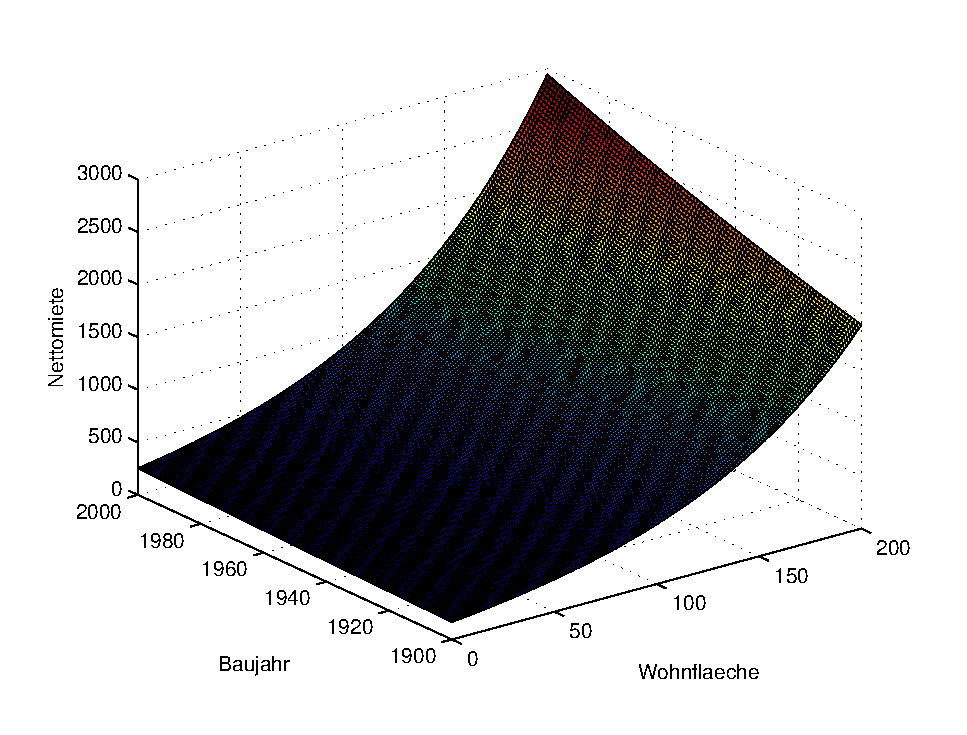
\includegraphics[width=10cm]{figures/nm_wfl_bj_log_approach}
  \end{center}

\end{frame}

\section{Ausblick}

\begin{frame}
  \frametitle{Ausblick}
  
  Im nächsten Vortrag folgt:
  \begin{itemize}
  \item Wie werden die Methoden angewendet
    \begin{itemize}
    \item Am Beispiel des Münchener Mietspiegels
    \end{itemize}
  \item Performance Analyse
    \begin{itemize}
    \item Wie verhalten sich die Algorithmen bei verschiedenen Datensätzen/Parametern 
    \end{itemize}
  \end{itemize}

\end{frame}

\end{document}
